\documentclass[11pt]{article}
\usepackage{graphicx}
\usepackage{fancyhdr}
% \usepackage{wrapfig}
\usepackage{hyperref}
\usepackage{tabularx}
\usepackage{setspace}
\usepackage{listings}

% math package
\usepackage{amsmath}
\usepackage{amssymb}

% matrix package
\usepackage{nicematrix}

% graph package
\usepackage{tikz}
\usetikzlibrary{positioning}


%\usepackage{yhmath}


% for R style
\usepackage{color}
\definecolor{mGreen}{rgb}{0,0.6,0}
\definecolor{mGray}{rgb}{0.5,0.5,0.5}
\definecolor{mPurple}{rgb}{0.58,0,0.82}
\definecolor{backgroundColour}{rgb}{0.95,0.95,0.92}


\lstdefinestyle{RStyle}{
    backgroundcolor=\color{backgroundColour},   
    commentstyle=\color{mGreen},
    keywordstyle=\color{magenta},
    numberstyle=\tiny\color{mGray},
    stringstyle=\color{mPurple},
    basicstyle=\footnotesize,
    breakatwhitespace=false,
    breaklines=true,
    captionpos=b,
    keepspaces=true,
    numbers=left,
    numbersep=5pt,
    showspaces=false,
    showstringspaces=false,
    showtabs=false,
    tabsize=2,
    language=R
}



\usepackage[spanish]{babel}
\decimalpoint

\newsavebox\CBox
\def\textBF#1{\sbox\CBox{#1}\resizebox{\wd\CBox}{\ht\CBox}{\textbf{#1}}}

\newenvironment{myenv}[1]
  {\begin{spacing}{#1}}
  {\end{spacing}}

\addtolength{\textwidth}{0.2cm}
\setlength{\parskip}{13pt}
\setlength{\parindent}{0.0cm}
\linespread{1.25}

\pagestyle{fancy}
\fancyhf{}
\rhead{TP Final - Sullivan}
\lhead{Probalidad y Estad\'istica}
\rfoot{\vspace{1cm} \thepage}

\renewcommand*\contentsname{\LARGE Índice}

\begin{document}

\begin{titlepage}
    \begin{center}
        \vfill
        \vfill
            \vspace{0.7cm}
            \noindent\textbf{\Huge Trabajo Pr\'actico Final}\par
            \noindent\textbf{\Huge Probabilidad y Estad\'istica}\par
            \vspace{.5cm}
        \vfill
        \noindent \textbf{\huge Alumna:}\par
        \vspace{.5cm}
        \noindent \textbf{\Large Sullivan, Katherine}\par

 
        \vfill
        \large Universidad Nacional de Rosario \par
        \noindent\large 2022
    \end{center}
\end{titlepage}
\par

\section*{Problema 1}
Tenemos un suceso cuya probabilidad de éxito es $p$. Realizamos intentos independientes de este suceso hasta obtener $k$ éxitos consecutivos. 
Definimos el proceso $N_k$, que denota el número de ensayos necesarios para obtener $k$ éxitos consecutivos.

a) Se nos solicita simular un cierto número de trayectorias del proceso $N_k$ (para el cual elegimos $k=4$) considerando un valor de $p < 0.5$ (para el cual consideramos $p=0.49$)

Simulamos 1000 realizaciones del proceso $N_4$ con $p=0.49$.

Para visualizar cuántas realizaciones fueron necesarias en cada caso para obtener 4 éxitos consecutivos de manera más ordenada presentamos una tabla de frecuencias que indica cuántas veces se necesitaron $x$ cantidad de sucesos para obtener 4 éxitos consecutivos.

\begin{center}
    \large\textbf{Cantidad de sucesos hasta obtener 4 éxitos consecutivos}
    
    \begin{tabularx} {0.7\textwidth}{ 
        | >{\raggedright\arraybackslash}X 
        | >{\raggedleft\arraybackslash}X 
        | >{\raggedleft\arraybackslash}X | }
        \hline
        \textbf{Cantidad de sucesos} & \textbf{Frecuencia absoluta} & \textbf{Frecuencia relativa} \\
        \hline
        4 & 64 & 0.064 \\ 
        \hline
        5 & 23 & 0.023 \\ 
        \hline
        6 & 29 & 0.029 \\ 
        \hline
        7 & 29 & 0.029 \\ 
        \hline
        8 & 31 & 0.031 \\ 
        \hline
        9 & 33 & 0.033 \\ 
        \hline
        10 & 27 & 0.027 \\ 
        \hline
        11 & 18 & 0.018 \\ 
        \hline
        12 & 33 & 0.033 \\ 
        \hline
        13 & 26 & 0.026 \\ 
        \hline
    \end{tabularx}    
    \begin{tabularx} {0.7\textwidth}{ 
        | >{\raggedright\arraybackslash}X 
        | >{\raggedleft\arraybackslash}X 
        | >{\raggedleft\arraybackslash}X | }
        \hline
        14 & 28 & 0.028 \\ 
        \hline
        15 & 11 & 0.011 \\ 
        \hline
        16 & 19 & 0.019 \\ 
        \hline
        17 & 25 & 0.025 \\ 
        \hline
        18 & 20 & 0.020 \\ 
        \hline
        19 & 20 & 0.020 \\ 
        \hline
        20 & 10 & 0.010 \\ 
        \hline
        21 & 20 & 0.020 \\ 
        \hline
        22 & 14 & 0.014 \\ 
        \hline
        23 & 14 & 0.014 \\ 
        \hline
        24 & 10 & 0.010 \\ 
        \hline
        25 & 9 & 0.009 \\ 
        \hline
        26 & 23 & 0.023 \\ 
        \hline
        27 & 12 & 0.012 \\ 
        \hline
        28 & 14 & 0.014 \\ 
        \hline
        29 & 12 & 0.012 \\ 
        \hline
        30 & 13 & 0.013 \\ 
        \hline
        31 & 12 & 0.012 \\ 
        \hline
        32 & 16 & 0.016 \\ 
        \hline
        33 & 11 & 0.011 \\ 
        \hline
        34 & 14 & 0.014 \\ 
        \hline
        35 & 18 & 0.018 \\ 
        \hline
        36 & 10 & 0.010 \\ 
        \hline
        37 & 11 & 0.011 \\ 
        \hline
        38 & 6 & 0.006 \\ 
        \hline
        39 & 13 & 0.013 \\ 
        \hline
        40 & 7 & 0.007 \\ 
        \hline
        41 & 9 & 0.009 \\ 
        \hline
        42 & 9 & 0.009 \\ 
        \hline
        43 & 5 & 0.005 \\ 
        \hline
        44 & 8 & 0.008 \\ 
        \hline
        45 & 9 & 0.009 \\ 
        \hline
        46 & 9 & 0.009 \\ 
        \hline
    \end{tabularx}    
    \begin{tabularx} {0.7\textwidth}{ 
        | >{\raggedright\arraybackslash}X 
        | >{\raggedleft\arraybackslash}X 
        | >{\raggedleft\arraybackslash}X | }
        \hline
        47 & 12 & 0.012 \\ 
        \hline
        48 & 6 & 0.006 \\ 
        \hline
        49 & 7 & 0.007 \\ 
        \hline
        50 & 8 & 0.008 \\ 
        \hline
        51 & 5 & 0.005 \\ 
        \hline
        52 & 6 & 0.006 \\ 
        \hline
        53 & 9 & 0.009 \\ 
        \hline
        54 & 7 & 0.007 \\ 
        \hline
        55 & 7 & 0.007 \\ 
        \hline
        56 & 7 & 0.007 \\ 
        \hline
        57 & 3 & 0.003 \\ 
        \hline
        58 & 10 & 0.010 \\ 
        \hline
        59 & 3 & 0.003 \\ 
        \hline
        60 & 5 & 0.005 \\ 
        \hline
        61 & 3 & 0.003 \\ 
        \hline
        62 & 1 & 0.001 \\ 
        \hline
        63 & 2 & 0.002 \\ 
        \hline
        64 & 4 & 0.004 \\ 
        \hline
        65 & 12 & 0.012 \\ 
        \hline
        66 & 3 & 0.003 \\ 
        \hline
        67 & 4 & 0.004 \\ 
        \hline
        68 & 3 & 0.003 \\ 
        \hline
        69 & 3 & 0.003 \\ 
        \hline
        70 & 9 & 0.009 \\ 
        \hline
        71 & 4 & 0.004 \\ 
        \hline
        72 & 6 & 0.006 \\ 
        \hline
        73 & 5 & 0.005 \\ 
        \hline
        74 & 2 & 0.002 \\ 
        \hline
        76 & 2 & 0.002 \\ 
        \hline
        77 & 3 & 0.003 \\ 
        \hline
        78 & 4 & 0.004 \\ 
        \hline
        79 & 4 & 0.004 \\ 
        \hline
        80 & 7 & 0.007 \\ 
        \hline
    \end{tabularx}    
    \begin{tabularx} {0.7\textwidth}{ 
        | >{\raggedright\arraybackslash}X 
        | >{\raggedleft\arraybackslash}X 
        | >{\raggedleft\arraybackslash}X | }
        \hline
        81 & 4 & 0.004 \\ 
        \hline
        82 & 4 & 0.004 \\ 
        \hline
        83 & 2 & 0.002 \\ 
        \hline
        84 & 2 & 0.002 \\ 
        \hline
        85 & 6 & 0.006 \\ 
        \hline
        87 & 2 & 0.002 \\ 
        \hline
        88 & 2 & 0.002 \\ 
        \hline
        89 & 3 & 0.003 \\ 
        \hline
        90 & 1 & 0.001 \\ 
        \hline
        91 & 2 & 0.002 \\ 
        \hline
        93 & 4 & 0.004 \\ 
        \hline
        94 & 2 & 0.002 \\ 
        \hline
        95 & 1 & 0.001 \\ 
        \hline
        96 & 2 & 0.002 \\ 
        \hline
        98 & 1 & 0.001 \\ 
        \hline
        99 & 1 & 0.001 \\ 
        \hline
        100 & 1 & 0.001 \\ 
        \hline
        101 & 1 & 0.001 \\ 
        \hline
        102 & 2 & 0.002 \\ 
        \hline
        103 & 2 & 0.002 \\ 
        \hline
        104 & 1 & 0.001 \\ 
        \hline
        107 & 2 & 0.002 \\ 
        \hline
        108 & 2 & 0.002 \\ 
        \hline
        112 & 1 & 0.001 \\ 
        \hline
        117 & 2 & 0.002 \\ 
        \hline
        119 & 1 & 0.001 \\ 
        \hline
        121 & 2 & 0.002 \\ 
        \hline
        126 & 1 & 0.001 \\ 
        \hline
        132 & 2 & 0.002 \\ 
        \hline
        135 & 1 & 0.001 \\ 
        \hline
        138 & 1 & 0.001 \\ 
        \hline
        139 & 1 & 0.001 \\ 
        \hline
        145 & 1 & 0.001 \\ 
        \hline
    \end{tabularx}    
    \begin{tabularx} {0.7\textwidth}{ 
        | >{\raggedright\arraybackslash}X 
        | >{\raggedleft\arraybackslash}X 
        | >{\raggedleft\arraybackslash}X | }
        \hline
        147 & 1 & 0.001 \\ 
        \hline
        160 & 1 & 0.001 \\ 
        \hline
        169 & 1 & 0.001 \\ 
        \hline
        176 & 1 & 0.001 \\ 
        \hline
        189 & 1 & 0.001 \\ 
        \hline
        191 & 1 & 0.001 \\ 
        \hline
        200 & 1 & 0.001 \\ 
        \hline \hline
        Total: & 1000 & 1\\
        \hline
    \end{tabularx}
\end{center}

Podemos ver entonces que la mínima cantidad de sucesos es 4 y la máxima 200. Que la mínima cantidad de sucesos sea 4 se mantendrá para cualquier realización del proceso, mientras que no hay un máximo fijo que se pueda establecer. 

También se puede apreciar que la mínima cantidad es la que presenta mayor frecuencia.

Para visualizar la infromación presentada en la tabla de manera más sintetizada e incluyendo medidas resúmenes relevantes como lo son la mediana y los cuartiles presentamos un boxplot con sus respectivas medidas resúmenes.

\begin{itemize}
    \item Primer cuartil: 11
    \item Mediana: 24
    \item Tercer cuartil: 46
    \item Rango intercuarti: 35
\end{itemize}

\begin{center}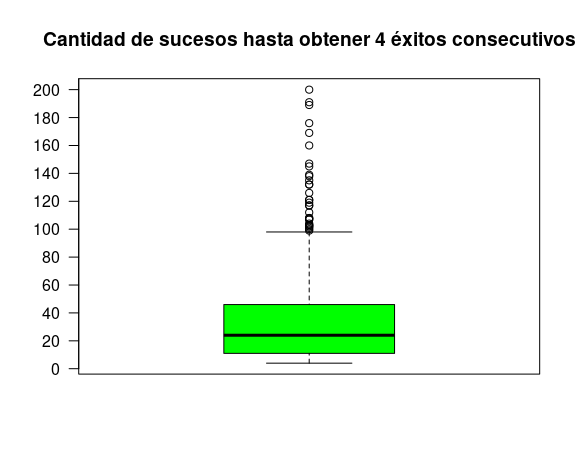
\includegraphics[scale = 0.65]{P1Boxplot.png}\end{center}

\vspace{-2cm}

b) A partir de la simulación realizada, estimamos la esperanza de $N_4$ sumando cada cantidad de sucesos multiplicado por su frecuencia relativa, resultando $E(N_4)=32.752$. 

\section*{Problema 2}

Consideramos el proceso $D_n =2\cdot I_n-1$, donde $D_n$ representa el cambio de posición de una partícula que se mueve a
lo largo de una línea recta con saltos de magnitud 1 en cada momento, ya que el mismo depende del
proceso Bernoulli $I_n$ : "la señal emitida en el momento $n$ es correcta".

Definimos $I_n$ tal que $I_n = 1$ si la señal emitida en el momento $n$ es correcta mientras que $I_n = 0$ en caso contrario, y definimos el estado inicial del proceso como $N_0 = 0$.

a) Se nos solicita simular 50 pasos de una trayectoria de $D_n$ para el proceso Bernoulli $I_n$ con un $p > 0.7$.

Para ello, elegimos $p=0.8$ y realizamos la simulación en R, obteniendo: 

\begin{align*}
    &D_n = [1, 1, 1, 1, 1, 1, 1, -1, 1, 1, -1, 1, 1, 1, 1, 1, -1, 1, 1, -1, 1, 1, 1, 1, 1, 1, 1, -1, -1, \\
    &1, 1, 1, 1, 1, 1, 1, 1, -1, 1, -1, 1, 1, 1, -1, 1, -1, 1, -1, -1, -1]
\end{align*}

b) Se nos solicita simular una realización del proceso $S_n$ : "posición de la partícula en el momento $n$".

Observamos que el proceso $S_n$: “posición de una particula en el momento $n$” es la suma
acumulada del proceso $D_n$.

Por lo tanto, una realización del proceso es: 

\vspace{-1.25cm}

\begin{align*}
    &S_n = [1, 2, 3, 4, 5, 6, 7, 6, 7, 8, 7, 8, 9, 10, 11, 12, 11, 12, 13, 12, 13, 14, 15, 16, 17, 18, 19, 18, 17, 18, \\
    &19, 20, 21, 22, 23, 24, 25, 24, 25, 24, 25, 26, 27, 26, 27, 26, 27, 26, 25, 24]
\end{align*}

\vspace{-0.65cm}

Para obtener una mejor idea del proceso y poder observar visualmente como la trayectoria tiene a infinito positivo (dado que $p$ es cercano a 1) realizamos un gráfico con la trayectoria.

\begin{center}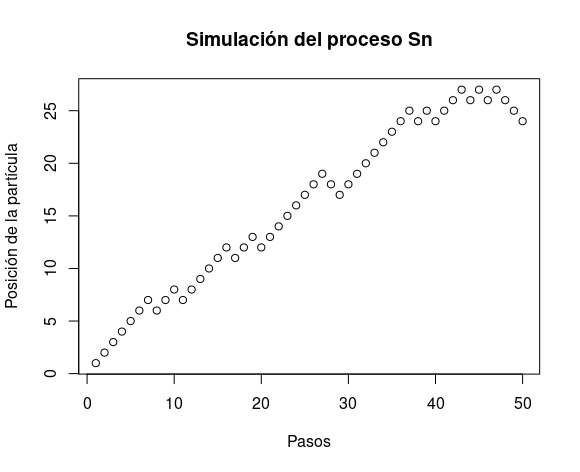
\includegraphics[scale = 0.6]{P2Simulacion.png}\end{center}


\section*{Problema 3}

Tenemos un jugador que tiene una apuesta inicial de k dólares y repetidamente apuesta 1 dólar en un juego
en el cual la probabilidad de ganar es p y la probabilidad de perder es 1-p. El estado inicial del proceso es $X_0= k$. 
Suponemos que el jugador decide detenerse cuando su fortuna alcanza $S$ dólares ($S > k$), o cae a $0$ dólar, lo que ocurra primero.

Consideramos, entonces, un proceso estocástico $N_n$ que representa el estado actual de la
apuesta de un jugador luego de $n$ juegos. El estado inicial del proceso es
$N_0 = k$, la apuesta inicial. Por cada juego, el jugador puede perder 1 o
ganar 1 de su apuesta. Por lo tanto podemos definir el proceso $X_n$ como
$X_n = 2 \cdot J_n - 1$, donde $J_n$ es el proceso de Bernoulli que representa: “el
n-ésimo juego se ganó", siendo $J_n=1$ cuando se ganó y $J_n=0$ en caso contrario.

a) Se nos solicita simular y visulizar la evolución del capital del jugador para un valor de $k$ y $S$ pero para distintos
valores de $p$ ($p < 0.5$, $p=0.5$ y $p> 0.5$).

Para eso elegimos $k=10$ y $S=30$ y realizamos la simulación con R.

\textbf{Caso $p < 0.5$:}

Para visualizar el caso $p < 0.5$ elegimos $p=0.25$. 

Observamos la siguiente evolución: 

\vspace{-1cm}

\begin{align*}
    [10, 11, 10, 9, 8, 9, 8, 9, 8, 7, 6, 5, 4, 3, 2, 3, 2, 1, 0]
\end{align*}

\vspace{-0.5cm}

que podemos apreciar mejor en el siguiente gráfico: 

\begin{center}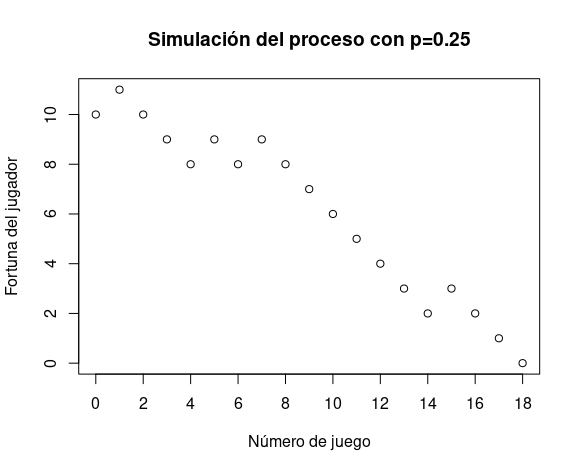
\includegraphics[scale = 0.51]{P3Sim1.png}\end{center}

\vspace{-0.25cm}

\textbf{Caso $p=0.5$:}

Observamos la siguiente evolución: 

\vspace{-1cm}

\begin{align*}
    &[10, 11, 10, 11, 12, 13, 14, 13, 12, 11, 10, 9, 8, 9, 8, 9, 8, 9, 8, 7, 6, 5, 6, 7, 6, 5, \\ 
    & 4, 5, 4, 3, 4, 3, 4, 5, 4, 5, 6, 5, 4, 3, 2, 3, 2, 3, 2, 3, 2, 1, 0]
\end{align*}

\vspace{-0.5cm}

que podemos apreciar mejor en el siguiente gráfico: 

\begin{center}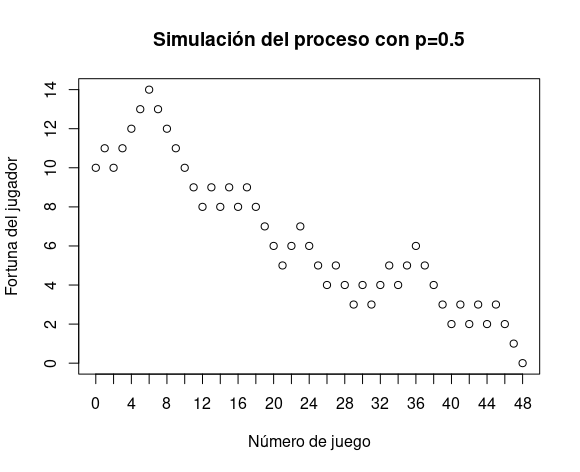
\includegraphics[scale = 0.55]{P3Sim2.png}\end{center}

\textbf{Caso $p > 0.5$:}

Para visualizar el caso $p > 0.5$ elegimos $p=0.75$. 

Observamos la siguiente evolución: 

\vspace{-1cm}

\begin{align*}
    & [10, 11, 12, 13, 14, 15, 14, 15, 14, 13, 14, 15, 16, 17, 18, 19, 20, 19, 20, 21, 22, 23, 24, \\ 
    & 25, 24, 25, 26, 27, 26, 27, 28, 29, 30]
\end{align*}

\vspace{-0.5cm}

que podemos apreciar mejor en el siguiente gráfico: 

\begin{center}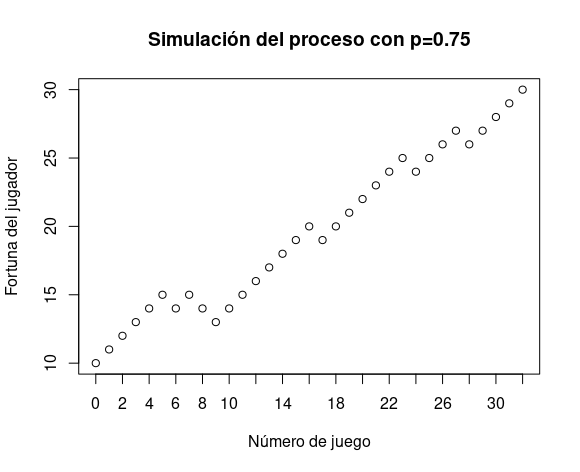
\includegraphics[scale = 0.55]{P3Sim3.png}\end{center}

b) Se nos solicita estimar, mediante la simulación de un número adecuado de trayectorias del capital del jugador, la
probabilidad de ruina de dicho jugador para los distintos escenarios planteados en a). 

Para eso, por cada escenario ($p=0.25$, $p=0.5$ y $p=0.75$) simulamos 10000 trayectorias del capital del jugador y observamos cuántas terminan en ruina para poder determinar la probabilidad indicada. 

\begin{itemize}
    \item Para $p=0.25$ la probabilidad de ruina es aproximadamente $1$.
    \item Para $p=0.5$ la probabilidad de ruina es aproximadamente $0.6658$.
    \item Para $p=0.75$ la probabilidad de ruina es aproximadamente $0$.
\end{itemize}


\section*{Problema 4}

Buscamos medir la efectividad del algoritmo Quicksort que opera sobre conjuntos,
midiendo la cantidad de comparaciones que realiza. Denominamos $M_n$ al
número esperado de comparaciones que realiza el algoritmo para un conjunto
de $n$ elementos.

a) Se nos solicita simular el algoritmo Quick-Sort para ordenar un conjunto de 7 números y calcular el número
promedio de comparaciones. 

Para lograr esto, simulamos 10000 veces el algoritmo Quick-Sort con distintas listas de 7 elementos y calculamos la cantidad de comparaciones en cada caso. 

Presentamos a continuación la tabla y un gráfico de barras que presentan con qué frecuencia se realizan $x$ comparaciones dentro de nuestras 10000 simulaciones.

\begin{center}
    \begin{tabularx} {0.7\textwidth}{ 
        | >{\raggedright\arraybackslash}X 
        | >{\raggedleft\arraybackslash}X | }
        \hline
        \textbf{Cantidad de comparaciones} & \textbf{Frecuencia absoluta} \\
        \hline
        10 & 141 \\
        \hline
        11 & 2114 \\
        \hline
        12 & 2019 \\
        \hline
        13 & 1700 \\
        \hline
        14 & 903 \\
        \hline
        15 & 1318 \\
        \hline
        16 & 548 \\
        \hline
        17 & 644 \\
        \hline
        18 & 239 \\
        \hline
        19 & 175 \\
        \hline
        20 & 85 \\
        \hline
        21 & 114 \\
        \hline \hline
        Total: & 10000 \\
        \hline
    \end{tabularx}
\end{center}

\begin{center}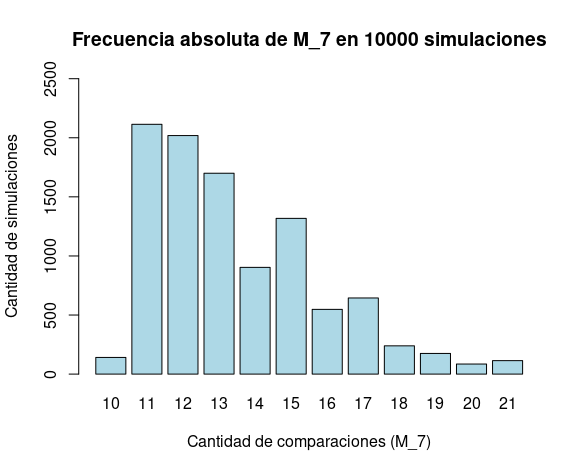
\includegraphics[scale = 0.6]{P4Barplot.png}\end{center}

Vemos aquí que el espacio muestral de $M_7$ resulta 
$$\{10,11,12,13,14,15,16,17,18,19,20,21\}$$

Calculando el promedio entre estas simulaciones obtenemos que es $13.4841$.

b) Se nos solicita explicitar cómo podríamos obtener el promedio de forma analítica, así que eso es lo que haremos a continuación. 

Sea una lista $l = [x_1, x_2, x_3, x_4, x_5, x_6, x_7]$. Se tiene la misma probabilidad de elegir cualquier $x_i, i = 1, \dots ,7$, por lo tanto esta probabilidad es $\frac{1}{n} = \frac{1}{7}$.

Luego de elegir un $x_i$, se realizan $n-1$ comparaciones, en este caso, $7$. Dependiendo la elección de $x_i$, se pueden generar diferentes listas a ordenar en el llamado recursivo:

\begin{itemize}
    \item 0 elementos menores a $x_i$ y 6 elementos mayores a $x_i$
    \item 1 elemento menor a $x_i$ y 5 elementos mayores a $x_i$
    \item 2 elementos menores a $x_i$ y 4 elementos mayores a $x_i$
    \item 3 elementos menores a $x_i$ y 3 elementos mayores a $x_i$
    \item 4 elementos menores a $x_i$ y 2 elementos mayores a $_i$
    \item 5 elementos menores a $x_i$ y 1 elemento mayor a $x_i$
    \item 6 elementos menores a $x_i$ y 0 elementos mayores a $x_i$
\end{itemize}

Sabemos que ordenar una lista vacía o con un elemento no requiere comparaciones, y que para ordenar una lista de 2 elementos se realiza 1 comparación. Además, ordenar una lista de $m$ elementos tiene el mismo costo, independientemente de sus elementos.

Por lo tanto, llegamos a que hay:

\begin{itemize}
    \item $\frac{2}{7}$ de probabilidad de ordenar una lista de 6 elementos
    \item $\frac{2}{7}$ de probabilidad de ordenar una lista de 5 elementos
    \item $\frac{2}{7}$ de probabilidad de ordenar una lista de 4 elementos y hacer una comparación más
    \item $\frac{1}{7}$ de probabilidad de ordenar dos listas de 3 elementos
\end{itemize}

Vemos que es necesario conocer la cantidad de comparaciones que se realizan sobre listas de 3, 4, 5 y 6 elementos.

Para \textbf{listas de 3 elementos}, luego de elegir un elemento al azar y realizar 2 comparaciones, hay $\frac{2}{3}$ de probabilidad de que se seleccione el menor o mayor elemento de la lista y por eso realizar 3 comparaciones en total (se le suma solo una comparación a las 2 iniciales), y hay $\frac{1}{3}$ de probabilidad de que se seleccione el elemento central, en cuyo caso no se deberan realizar más comparaciones, debiendo realizar 2 comparaciones en total.

Para \textbf{listas de 4 elementos}, luego de elegir un elemento al azar y realizar 3 comparaciones, hay $\frac{1}{2}$ de probabilidad de que se seleccione el menor o mayor elemento de la lista y que reste ordenar una lista de 3 elementos, y hay $\frac{1}{2}$ de probabilidad de que se haga 1 comparación más por haber elegido alguno de los elementos centrales.

Multiplicando estas probabilidades con lo obtenido para listas de 3 elementos, se obtiene que para listas de 4 elementos hay:

\begin{itemize}
    \item $\frac{1}{2}$ de probabilidad de que se realicen 4 comparaciones
    \item $\frac{1}{6}$ de probabilidad de que se realicen 5 comparaciones
    \item $\frac{1}{3}$ de probabilidad de que se realicen 6 comparaciones
\end{itemize}

Para \textbf{listas de 5 elementos}, tenemos que hacer un análisis un poco más preciso: 

En una primer instacia tenemos que para una lista de 5 elementos hay: 

\begin{itemize}
    \item $\frac{2}{5}$ de probabilidad de ordenar una lista de 4 elementos
    \item $\frac{2}{5}$ de probabilidad de ordenar una lista de 3 elementos
    \item $\frac{1}{5}$ de probabilidad de realizar 2 comparaciones
\end{itemize}

y, por lo que analizamos anteriormente para las listas de 3 y 4 elementos, obtenemos entonces que para listas de 5 elementos hay: 

\begin{itemize}
    \item $\frac{1}{3}$ de probabilidad de que se realicen 6 comparaciones
    \item $\frac{4}{15}$ de probabilidad de que se realicen 7 comparaciones
    \item $\frac{1}{5}$ de probabilidad de que se realicen 8 comparaciones
    \item $\frac{1}{15}$ de probabilidad de que se realicen 9 comparaciones
    \item $\frac{2}{15}$ de probabilidad de que se realicen 10 comparaciones
\end{itemize}

Y por último, para \textbf{listas de 6 elementos} en una primera instancia tenemos que: 

\begin{itemize}
    \item $\frac{2}{6}$ de probabilidad de ordenar una lista de 5 elementos
    \item $\frac{2}{6}$ de probabilidad de ordenar una lista de 4 elementos
    \item $\frac{2}{6}$ de probabilidad de ordenar una lista de 3 elementos y tener que hacer una comparación más
\end{itemize}

y por lo que analizamos anteriormente para las listas de 3, 4 y 5 elementos tenemos que para listas de 6 elementos hay: 

\begin{itemize}
    \item $\frac{2}{9}$ de probabilidad de que se realicen 11 comparaciones
    \item $\frac{4}{45}$ de probabilidad de que se realicen 12 comparaciones
    \item $\frac{1}{15}$ de probabilidad de que se realicen 13 comparaciones
    \item $\frac{1}{45}$ de probabilidad de que se realicen 14 comparaciones
    \item $\frac{2}{45}$ de probabilidad de que se realicen 15 comparaciones
    \item $\frac{7}{18}$ de probabilidad de que se realicen 9 comparaciones
    \item $\frac{1}{18}$ de probabilidad de que se realicen 10 comparaciones
    \item $\frac{1}{9}$ de probabilidad de que se realicen 8 comparaciones
\end{itemize}

Entonces, volviendo a nuestro análisis principal de las comparaciones necesarias para ordenar nuestro conjunto de 7 elementos. 

Dividiremos según los casos expuestos anteriormente, para hacer el análisis más llevadero.

Habíamos establecido que tenemos $\frac{2}{7}$ de probabilidad de ordenar una lista de 6 elementos. Esto quiere decir que tenemos: 

\begin{itemize}
    \item $\frac{4}{63}$ de probabilidad de que se realicen 17 comparaciones
    \item $\frac{8}{315}$ de probabilidad de que se realicen 18 comparaciones
    \item $\frac{2}{105}$ de probabilidad de que se realicen 19 comparaciones
    \item $\frac{2}{315}$ de probabilidad de que se realicen 20 comparaciones
    \item $\frac{4}{315}$ de probabilidad de que se realicen 21 comparaciones
    \item $\frac{1}{9}$ de probabilidad de que se realicen 15 comparaciones
    \item $\frac{1}{63}$ de probabilidad de que se realicen 16 comparaciones
    \item $\frac{2}{63}$ de probabilidad de que se realicen 14 comparaciones
\end{itemize}

A su vez, establecimos que tenemos $\frac{2}{7}$ de probabilidad de tener que ordenar una lista de 5 elementos. Esto quiere decir que tenemos: 

\begin{itemize}
    \item $\frac{2}{21}$ de probabilidad de que se realicen 12 comparaciones
    \item $\frac{8}{105}$ de probabilidad de que se realicen 13 comparaciones
    \item $\frac{2}{35}$ de probabilidad de que se realicen 14 comparaciones
    \item $\frac{2}{105}$ de probabilidad de que se realicen 15 comparaciones
    \item $\frac{4}{105}$ de probabilidad de que se realicen 16 comparaciones
\end{itemize}

También, establecimos que tenemos $\frac{2}{7}$ de probabilidad de tener que ordenar una lista de 4 elementos y hacer una comparación más. Esto quiere decir que tenemos: 

\begin{itemize}
    \item $\frac{1}{7}$ de probabilidad de que se realicen 11 comparaciones
    \item $\frac{1}{21}$ de probabilidad de que se realicen 12 comparaciones
    \item $\frac{2}{21}$ de probabilidad de que se realicen 13 comparaciones
\end{itemize}

Y, por último, establecimos que tenemos $\frac{1}{7}$ de probabilidad de ordenar dos listas de 3 elementos. Esto quiere decir que tenemos:

\begin{itemize}
    \item $\frac{4}{63}$ de probabilidad de que se realicen 11 comparaciones (2 posibilidades de 1 lista con 3 comparaciones y la otra con 2)
    \item $\frac{4}{63}$ de probabilidad de que se realicen 12 comparaciones (2 listas con 3 comparaciones)
    \item $\frac{1}{63}$ de probabilidad de que se realicen 10 comparaciones (2 listas con 2 comparaciones)
\end{itemize}

Ahora unamos estos análisis parciales y veamos que para ordenar una lista de 7 elementos tenemos: 

\begin{itemize}
    \item $\frac{1}{63}$ de probabilidad de que se realicen 10 comparaciones
    \item $\frac{13}{63}$ de probabilidad de que se realicen 11 comparaciones
    \item $\frac{13}{63}$ de probabilidad de que se realicen 12 comparaciones
    \item $\frac{6}{35}$ de probabilidad de que se realicen 13 comparaciones
    \item $\frac{4}{45}$ de probabilidad de que se realicen 14 comparaciones
    \item $\frac{41}{315}$ de probabilidad de que se realicen 15 comparaciones
    \item $\frac{17}{315}$ de probabilidad de que se realicen 16 comparaciones
    \item $\frac{4}{63}$ de probabilidad de que se realicen 17 comparaciones
    \item $\frac{8}{315}$ de probabilidad de que se realicen 18 comparaciones
    \item $\frac{2}{105}$ de probabilidad de que se realicen 19 comparaciones
    \item $\frac{2}{315}$ de probabilidad de que se realicen 20 comparaciones
    \item $\frac{4}{315}$ de probabilidad de que se realicen 21 comparaciones
\end{itemize}

Calculando el promedio, obtenemos entonces que este es $13.4857$. Con lo que vemos que la aproximación generada por la simulación en a) resulta bastante precisa.

\section*{Problema 5}

Tenemos una red con 7 páginas. Por el algoritmo Page-Rank la "importancia" de cada página está determinada por la probabilidad de que un usuario se encuentre en la página luego de un tiempo navegando entre páginas accediendo a las siguientes mediantes los enlaces de hipertexto que tiene la página dónde se encontraba. 
Si una página cuenta con más de 1 enlace de hipertexto se distribuye la importancia de la página entre todas para las cuales tiene un enlace.

a) Se nos solicita modelar el comportamiento de visitas a las páginas como una cadena de Markov. 

Tomando la Figura 1, armamos la siguiente cadena de Markov con su respectiva matriz de transición en un paso.

% GRAFO
\begin {center}
\begin {tikzpicture}[-latex, auto, node distance = 4 cm and 5cm, on grid, semithick, state/.style = {circle, color = white, draw, black, text = black, minimum width = 1 cm}]
\node[state] (F) {$f$};
\node[state] (E) [above right = of F] {$e$};
\node[state] (B) [above left = of F] {$b$};
\node[state] (G) [right = of F] {$g$};
\node[state] (C) [below left = of F] {$c$};
\node[state] (D) [below right = of F] {$d$};
\node[state] (A) [above = of F] {$a$};
\path (C) edge node[below = 0.15 cm] {$1/2$} (F);
\path (C) edge node[below = 0.15 cm] {$1/2$} (D);
\path (D) edge node[below = 0.15 cm] {$1$} (F);
\path (B) edge node[below = 0.15 cm] {$1/3$} (A);
\path (B) edge node[below = 0.15 cm] {$1/3$} (C);
\path (B) edge [bend right = 15] node[below = 0.15 cm] {$1/3$} (F);
\path (F) edge [bend right = 15] node[below = 0.15 cm] {$1/2$} (B);
\path (F) edge [bend right = 15] node[below = 0.15 cm] {$1/2$} (A);
\path (A) edge [bend right = 15] node[below = 0.15 cm] {$1/2$} (F);
\path (A) edge [bend right = 15] node[below = 0.15 cm] {$1/2$} (E);
\path (E) edge [bend right = 15] node[below = 0.15 cm] {$1/4$} (A);
\path (E) edge [bend right = 15] node[below = 0.15 cm] {$1/4$} (G);
\path (E) edge node[below = 0.15 cm] {$1/4$} (F);
\path (E) edge [bend left = 25] node[below = 0.15 cm] {$1/4$} (D);
\path (G) edge node[below = 0.15 cm] {$1/6$} (D);
\path (G) edge [bend right = 15] node[below = 0.15 cm] {$1/6$} (E);
\path (G) edge node[below = 0.15 cm] {$1/6$} (C);
\path (G) edge node[below = 0.15 cm] {$1/6$} (F);
\path (G) edge [bend left = 25] node[below = 0.15 cm] {$1/6$} (A);
\path (G) edge [bend left = 65] node[below = 0.15 cm] {$1/6$} (B);
\end{tikzpicture}
\end{center}

% MATRIZ
\begin{equation}
    P = \begin{pNiceMatrix}[first-row,first-col]
              & a   & b   & c   & d   & e   & f   & g   \\
            a & 0   & 0   & 0   & 0   & 1/2 & 1/2 & 0   \\
            b & 1/3 & 0   & 1/3 & 0   & 0   & 1/3 & 0   \\
            c & 0   & 0   & 0   & 1/2 & 0   & 1/2 & 0   \\
            d & 0   & 0   & 0   & 0   & 0   & 1   & 0   \\
            e & 1/4 & 0   & 0   & 1/4 & 0   & 1/4 & 1/4 \\
            f & 1/2 & 1/2 & 0   & 0   & 0   & 0   & 0   \\
            g & 1/6 & 1/6 & 1/6 & 1/6 & 1/6 & 1/6 & 0   \\
        \end{pNiceMatrix}
\end{equation}

b) Se nos solicita simular 100 pasos para visualizar una trayectoria de este proceso. 

Hacemos la simulación en R, eligiendo aleatoriamente la página inicial y a continuación presentamos un gráfico que simula la trayectoria

\begin{center}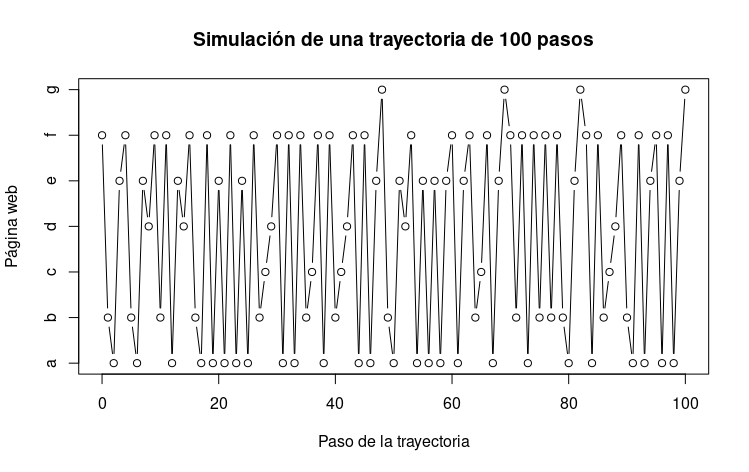
\includegraphics[scale = 0.65]{P5Sim.png}\end{center}

\vspace{-0.5cm}

Resulta interesante también analizar la frecuencia con la cuál se visitaron las distintas páginas, para tener una idea de su importancia. Por lo tanto, realizamos un gráfico de barras que presenta las veces que se visitó cada una de las páginas. 

\begin{center}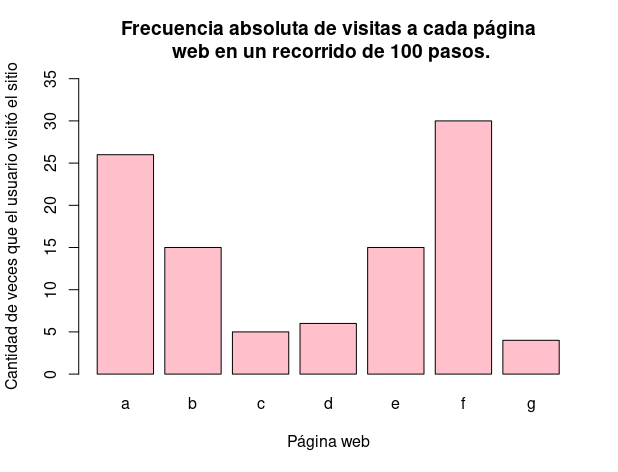
\includegraphics[scale = 0.55]{P5Barplot.png}\end{center}

c) Se nos solicita determinar el rango de cada página.

Para lograrlo debemos calcular la distribución invariante $\pi$, la cual podemos asegurar que existe y es única puesto que la cadena es cerrada, finita, irreducible y aperiódica. 

Para calcular $\pi$ debemos plantear las ecuaciones de equilibrio y la ecuación normalizadora y resolver el sistema de ecuaciones formado por ellas. 

El sistema de ecuaciones es, entonces el siguiente: 

\begin{equation*}
    \begin{cases}
        \pi_a = \frac{1}{3} \cdot \pi_b + \frac{1}{4} \cdot \pi_e + \frac{1}{2} \cdot \pi_f + \frac{1}{6} \cdot \pi_g \\
        \pi_b = \frac{1}{2} \cdot \pi_f + \frac{1}{6} \cdot \pi_g \\
        \pi_c = \frac{1}{3} \cdot \pi_b + \frac{1}{6} \cdot \pi_g \\
        \pi_d = \frac{1}{2} \cdot \pi_c + \frac{1}{4} \cdot \pi_e + \frac{1}{6} \cdot \pi_g \\
        \pi_e = \frac{1}{2} \cdot \pi_a + \frac{1}{6} \cdot \pi_g \\
        \pi_f = \frac{1}{2} \cdot \pi_a + \frac{1}{3} \cdot \pi_b + \frac{1}{2} \cdot \pi_c + \pi_d + \frac{1}{4} \cdot \pi_e + \frac{1}{6} \cdot \pi_g \\
        \pi_g = \frac{1}{4} \cdot \pi_e \\
        \pi_a + \pi_b + \pi_c + \pi_d + \pi_e + \pi_f + \pi_g = 1 \\
    \end{cases}
\end{equation*}

Resolviéndolo obtenemos entonces que: 

\vspace{-0.5cm}

\begin{equation*}
    \pi = \begin{pmatrix}
        0.2453 & 0.16 & 0.0587 & 0.0667 & 0.128 & 0.3093 & 0.032 \\
    \end{pmatrix}
\end{equation*}

Y por lo tanto: 

\vspace{-0.3cm}

\begin{itemize}
    \item el rango de a es 0.2453
    \item el rando de b es 0.16
    \item el rango de c es 0.0587
    \item el rango de d es 0.0667
    \item el rango de e es 0.128
    \item el rango de f es 0.3093
    \item el rango de g es 0.032
\end{itemize}

\section*{Problema 6}

Tenemos bajo estudio el número de vuelos que recibe un aeropuerto a una tasa
$\lambda$ (aterrizajes/hora).

a) Se nos plantea que el aeropuerto recibe vuelos comenzando a las 2 am a una tasa de 3 aterrizajes por hora, de
acuerdo a un Proceso Poisson y se nos solicita simular el comportamiento de dicho proceso durante 24 horas y
graficar la trayectoria obtenida.

Para realizar una simulación primero generamos un número aleatorio $n$ de la distribucion de Poisson con parámetro
$\lambda \cdot t$ (donde t es el tiempo total). Este va a representar la cantidad de eventos 
que ocurren en el tiempo $t$ en un Proceso de Poisson a una tasa $\lambda$. Luego generamos $n$ valores 
de la distribución uniforme (pues, la probabilidad de que un evento ocurra a un momento determinado
es la misma para cada evento) entre el $t$ inicial y el final. Estos son los instantes donde ocurre un evento.

Realizamos la simulación planteada en R y obtuvimos el siguiente gráfico.

\begin{center}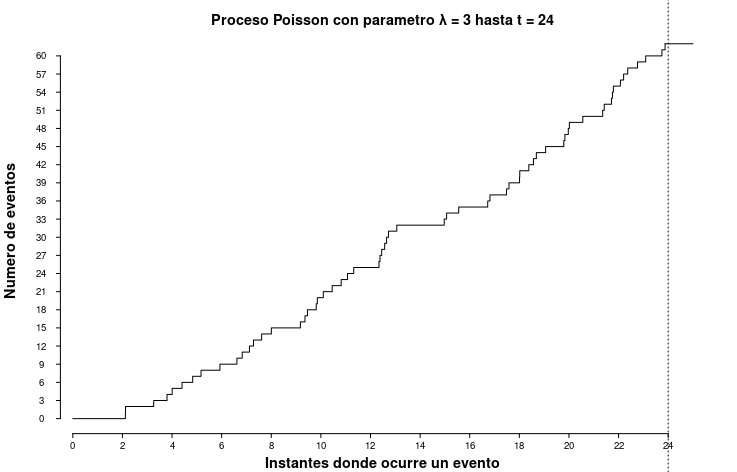
\includegraphics[scale = 0.67]{P6Sim.png}\end{center}

b) Ahora se nos solicita simular una trayectoria muestral durante un intervalo de tiempo suficientemente largo $[0,T]$ y calcular
los tiempos entre llegadas para luego representarlos gráficamente a través
de un histograma y comentar cuál es el modelo apropiado para para describir esa variable.

Para ello elegimos $T=4000$ y realizamos la simulación. Una vez obtenidos los instantes en los
que ocurre cada evento, calculamos las diferencias entre cada par de instantes consecutivos, obteniendo así los tiempos entre-arribos. Presentamos la información en el siguiente histograma. 

\begin{center}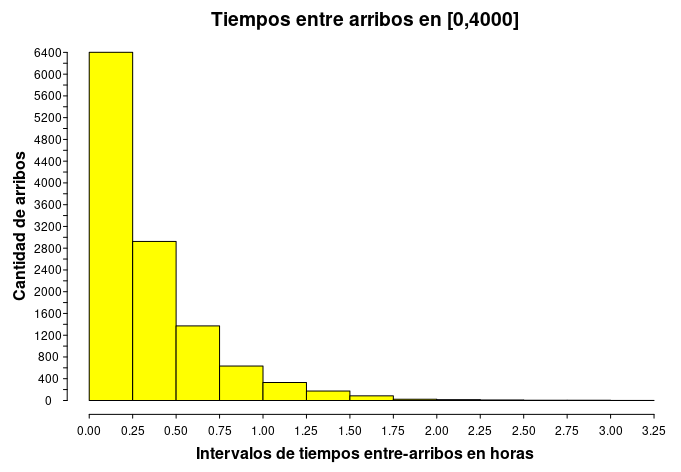
\includegraphics[scale = 0.65]{P6Histo.png}\end{center}

Podemos ver que el tiempo transcurrido entre dos arribos es independiente de los instantes de los arribos
previos (y de los arribos de los que se trate).

El modelo apropiado para describir esta variable es el de la distribución exponencial. 

% mean 1/lambda -> 3

\section*{Problema 7}

Tenemos un honeypot, cuyos datos son estudiados utilizando cadenas de Markov. Observamos ataques 
contra cuatro puertos de computadoras (80, 135, 139 y 445) durante un año. 

Los estados de la cadena de Markov son los cuatro puertos y se incluye un nodo (N/A) indicando que ningún puerto está siendo atacado. Los datos de monitorean
semanalmente y el puerto más atacado durante la semana es guardado. La matriz de transición para la
cadena estimada para los ataques semanales es:

\begin{equation*}
    P = \begin{pNiceMatrix}[first-row,first-col]
                & 80   & 135  & 139  & 445  & NA   \\
            80  & 0    & 0    & 0    & 0    & 1    \\
            135 & 0    & 8/13 & 3/13 & 1/13 & 1/13 \\
            139 & 1/16 & 3/16 & 3/8  & 1/4  & 1/8  \\
            445 & 0    & 1/11 & 4/11 & 5/11 & 1/11 \\
            NA  & 0    & 1/8  & 1/2  & 1/8  & 1/4  \\
        \end{pNiceMatrix}
\end{equation*}

con distribución inicial $\pi_0 = (0,0,0,0,1)$.

a) Se nos solicita determinar cuáles son los puertos con más y menos probabilidad de ser
atacados luego de 3 semanas. 

Como $P$ es la matríz de transición en un paso (una semana) y $\pi_0$ la distribución inicial, 
podemos determinar la distribución de probabilidad de que los puertos sean atacados luego de 3 semanas
con $\pi_0 * P^3$. 

Obtenemos entonces

\begin{equation*}
    \pi_0 * P^3 = \begin{pNiceMatrix}[first-row]
        80         & 135       & 139       & 445      & NA        \\
        0.02417504 & 0.2422698 & 0.3482356 & 0.232574 & 0.1527455 \\
    \end{pNiceMatrix}
\end{equation*}

Por lo tanto, tenemos que el puerto 80 es el de menor probabilidad de ser atacado y el puerto 139 es el de mayor probabilidad de ser atacado. 

b) Se nos solicita encontrar la distribución límite (si es que existe) de los puertos atacados.

Como $E = \{80, 135, 139, 445, NA\}$ es un conjunto cerrado, irreducible y finito, deducimos que sus elemento son estados positivamente recurrentes. 
Además, tenemos que los estados son aperiódicos. Por lo tanto, la cadena es ergódica.

Como la cadena es finita y ergódica sabemos que existe la distribución invariante. Para obtenerla planteamos el correspondiente sistema de ecuaciones: 


\begin{equation*}
    \begin{cases}
        \pi_{80} = \frac{1}{16} \cdot \pi_{139} \\
        \pi_{135} = \frac{8}{13} \cdot \pi_{135} + \frac{3}{16} \cdot \pi_{139} + \frac{1}{11} \cdot \pi_{445} + \frac{1}{8} \cdot \pi_{NA} \\
        \pi_{139} = \frac{3}{13} \cdot \pi_{135} + \frac{3}{8} \cdot \pi_{139} + \frac{4}{11} \cdot \pi_{445} + \frac{1}{2} \cdot \pi_{NA} \\
        \pi_{445} = \frac{1}{13} \cdot \pi_{135} + \frac{1}{4} \cdot \pi_{139} + \frac{5}{11} \cdot \pi_{445} + \frac{1}{8} \cdot \pi_{NA} \\
        \pi_{NA} = \pi_{80} + \frac{1}{13} \cdot \pi_{135} + \frac{1}{8} \cdot \pi_{139} + \frac{1}{11} \cdot \pi_{445} + \frac{1}{4} \cdot \pi_{NA} \\
        \pi_{80} + \pi_{135} + \pi_{139} + \pi_{445} + \pi_{NA} = 1 \\
    \end{cases}
\end{equation*}

Resuelto obtenemos la distribución límite de los puertos atacados:

\begin{equation*}
    \pi = \begin{pNiceMatrix}[first-row]
        80     & 135    & 139    & 445    & NA     \\
        0.0215 & 0.2669 & 0.3435 & 0.2273 & 0.1408 \\
    \end{pNiceMatrix}
\end{equation*}


\end{document}